\documentclass{sig-alternate}
\usepackage[section]{algorithm}
%\usepackage[]{algorithm2e}
\usepackage{algorithmic}
\usepackage{balance}
\usepackage{makecell}
\usepackage[usenames,dvipsnames]{color}
\usepackage[10pt]{moresize}
\usepackage[font=small,skip=0pt]{caption}
\usepackage{dblfloatfix}

\setlength{\abovecaptionskip}{10pt plus 0pt minus 2pt}
%\newenvironment{definition}{\begin{defn}\begin{em}}{\end{em}\end{defn}}
\newcommand{\inred}[1]{{\color{BrickRed}\sf\textbf{\textsc{#1}}}}
\newcommand{\card}[1]{|#1|}
\newcommand{\norm}[1]{\left\lVert#1\right\rVert}
\newcommand{\bfd}{\mathbf{d}}
\newcommand{\bfu}{\mathbf{u}}
\newcommand{\bfq}{\mathbf{q}}
\newcommand{\Z}{\mathbb{Z}}
\DeclareMathOperator*{\argmin}{arg\,min}
\DeclareMathOperator*{\argmax}{arg\,max}
\newtheorem{definition}{Definition}
\newtheorem{theorem}{Theorem}[section]
\newtheorem{thm}{Theorem}[section]
\newtheorem{lemma}[theorem]{Lemma}
\newtheorem{proposition}[theorem]{Proposition}
\newtheorem{corollary}[theorem]{Corollary}
\newtheorem{Assumption}[theorem]{Assumption}
\newtheorem{Condition}[theorem]{Condition}
\newtheorem{exe}
[thm]{Exercise}
\newtheorem{eg}[thm]{Example}
\newtheorem{conj}[thm]{Conjecture}
\newcommand{\comment}[1]{\frameit{Comment}{#1}}%
\newcommand{\note}[1]{\frameit{Note}{#1}}
\newcommand{\todo}[1]{\frameit{To-do}{#1}}
\newcommand{\inote}[1]{\inred{$<<<${#1}$>>>$}}
\newcommand{\frameit}[2]{
    \begin{center}
    {\color{BrickRed}
    \framebox[3.3in][l]{
        \begin{minipage}{3in}
        \inred{#1}: {\sf\color{Black}#2}
        \end{minipage}
    }\\
    }
    \end{center}
}

\begin{document}

\sloppy
\newcommand{\para}[1]{\par \bigskip \noindent {\bf #1.}}
\newcommand{\spara}[1]{\par \bigskip \noindent {\sc #1.}}

\newcommand{\ymatrix}[1]{\mathbf{#1}}
\newcommand{\yvector}[1]{\mathbf{#1}}
\newcommand{\ytrans}[1]{#1^{\mathsf{T}}}

\newcommand{\yset}[1]{\mathcal{#1}}
\long\def\/*#1*/{}
%

\title{Click-Based Content Recommendation for Hierarchical Semantic Streams}
%\subtitle{[Extended Abstract]
%\titlenote{A full version of this paper is available as
%\textit{Author's Guide to Preparing ACM SIG Proceedings Using
%\LaTeX$2_\epsilon$\ and BibTeX} at
%\texttt{www.acm.org/eaddress.htm}}}
%
% You need the command \numberofauthors to handle the "boxing"
% and alignment of the authors under the title, and to add
% a section for authors number 4 through n.
%
% Up to the first three authors are aligned under the title;
% use the \alignauthor commands below to handle those names
% and affiliations. Add names, affiliations, addresses for
% additional authors as the argument to \additionalauthors;
% these will be set for you without further effort on your
% part as the last section in the body of your article BEFORE
% References or any Appendices.

%\numberofauthors{3}
%\author{
%\alignauthor John Jiang \\
%\affaddr{Yahoo! Labs}\\
%\affaddr{Sunnyvale, CA, USA}\\
%\email{\normalsize jyj@yahoo-inc.com}\\
%\alignauthor Ruiqiang Zhang\\
%\affaddr{Yahoo! Labs}\\
%\affaddr{Sunnyvale, CA, USA}\\
%\email{\normalsize ruiqiang@yahoo-inc.com}\\
%\alignauthor Youssef Billawal \\
%\affaddr{Yahoo! Labs}\\
%\affaddr{Sunnyvale, CA, USA}\\
%\email{\normalsize billawal@yahoo-inc.com}\\
%}

\maketitle
\begin{abstract}

We design a unified recommendation system for hierarchical personalized news 
streams, using three sequential phases to optimize for serving-time 
efficiency. Within each phase we use user click count feedbacks as training 
signals. This solves the issue of insufficient training labels in the context 
of content multi-classification (phase 0). In the personalization stage, we 
judiciously balance multilinear regression (phase 1) with gradient boosting 
models (phase 2) to ensure coverage, recency, and relevance at the same time, 
while maintaining low latency. The models include various features inspired by 
recency, personalization, popularity, and target stream. Significant 
improvements are observed in both offline experiments and online bucket test. 

\end{abstract}

% A category with only the three required fields
\category{H.3.m}{Information Search and Retrieval}{Miscellaneous}

\terms{Algorithms, Information Retrieval}

\keywords{News  recommendation, Information retrieval, Personalization, Semantic stream classifier, Multi-stream recommendation, Recency}


\section{Introduction}



Developing efficient and accurate personalized recommendation systems of 
news-worthy content has been a focus of today's media industry. 
On the one hand search engines have enabled users to locate articles or 
multimedia content of any topic within a few keystrokes. On the other hand, 
users are constantly overwhelmed by the amount of information generated 
daily, much of which is irrelevant to their personal interest. Thus 
directory-style news streams organized by topics are becoming increasingly 
popular. 

Under the latter framework, we not only need to recommend generically interesting articles, but those within a specific category, such as sports, finance, or technology, to a diverse array of users. Underneath each broad category lies more sub-categories that facilitate users to find relevant and interesting content quickly (Figure~\ref{hierarchy}).
\begin{figure*}
\centering
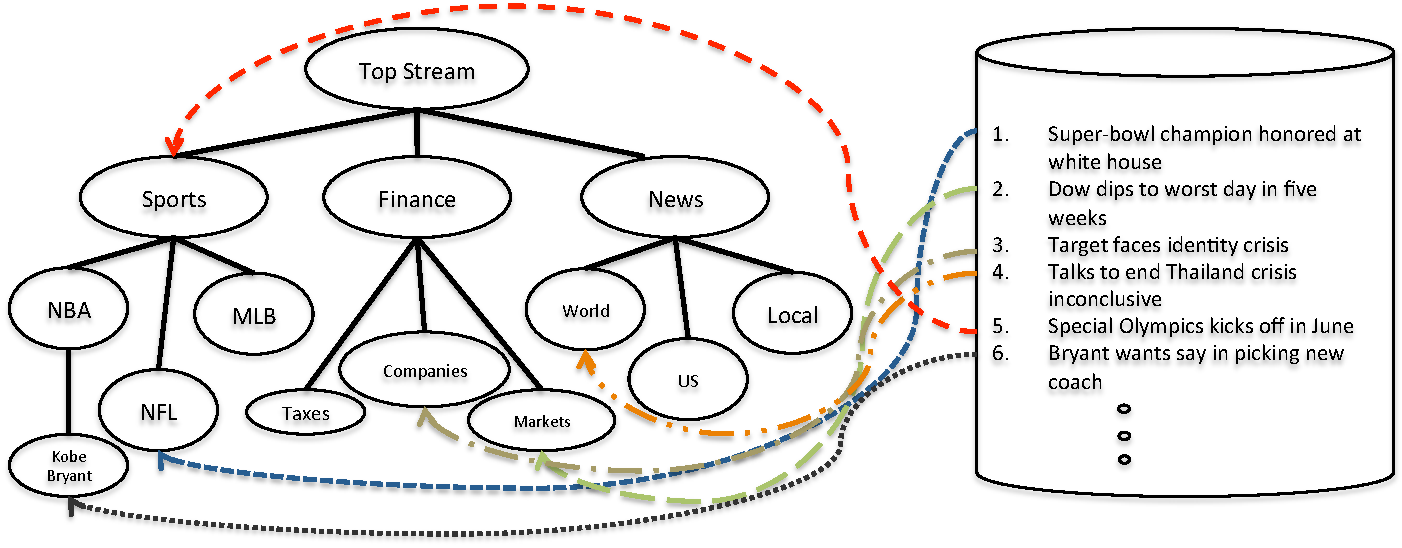
\includegraphics[scale=0.7]{Hierarchy.pdf}
\caption{Semantic Stream Hierarchy} \label{hierarchy}
\end{figure*}

Different from traditional news recommendation for a single stream, the first 
challenge is to assign articles into corresponding semantic streams as shown 
in the figure. One obvious approach is to implement a document filter for each 
category node on the content hierarchy.  However, the semantic streams are not 
static structures. It is evolving. New nodes may be added by any reasons such 
as sports (Olympics games), natural disasters (MH370) or political events 
(obamacare). To train a new document filter requires the labeling of training 
examples. Given the number of streams (easily in the 1000's) in question and 
its dynamic property, it is impossible to solve it by editorial resource.
But document filter is still useful as a starting point. We address the 
problem with a combination of user click feedbacks and editorial labeling.


Even after the filter problem is solved, users visiting different category 
streams can have very different sets of browsing interests. Furthermore, 
articles that are popular in a general stream may be less popular in a 
substream, and vice versa. While lower streams give more accurate user intent, 
higher streams provide more abundant user feedback. Each stream therefore may 
require its own personalization and ranking model for optimal user experience. 
Scalability is again a major practical concern here. In addition, many streams 
have very limited user statistics to build a meaningful and robust model, 
which suggests that we take a holistic approach by combining streams at lower 
branches of the hierarchy for model training.

Justified by the above reasoning, we therefore propose a system design with 
essentially 2 components: a category stream filter based on linear classifier 
(phase 0) followed by a personalization and ranking machine. Due to runtime 
constraints, the latter is further subdivided into two phases, with phase 1 
selecting among hundreds of thousands of articles only the top 200 candidates 
according to stream relevance and user preferences, using a simple linear 
model with only positive weights (negative pruning). The features consist of 
entity scores within the user and document profile, the popularity score of 
the article, measured in terms of discounted click-through rate(CTR), and 
finally the freshness of the content. Phase 2 then performs re-ranking of 
those 200 articles using the more sophisticated Gradient Boosted Decision Tree 
(GBDT) model, and integrating tens of new features including a content type 
feature that is unique for multiple semantic stream ranking.  
%Finally phase 3 takes into account pairwise similarity of those 200 articles and slightly reorganize them to achieve better diversification. 
Altogether, the three phases yield an efficient approximate solution to the optimal ranking problem; an exact solution is clearly too expensive for any reasonably sized content/user pools.

The paper is organized as follows. Stream classifier is described in 
section~\ref{sec:system design} including feature source discussion 
(\ref{sec:feature engineering}), stream classifier(section~\ref{sec:stream 
classifier}), Phase 1 ranking (\ref{sec:phase1 ranking}) and Phase 2 ranking 
(\ref{sec:phase2}). Experimental results are in section~\ref{sec:experiments} 
where we describes metrics, phase 0, phase 1 and phase 2 results. 
Section~\ref{sec:conclusions} concludes the paper.


%One of the earliest prototypes of personalized ranking system is based on a 
%simple linear matching model of user interest profile and document topic 
%profile. This crude approach has proved effective in promoting highly relevant 
%articles, videos or slideshows to each individual user, even when we have only 
%accumulated partial information about the user. Unfortunately there are 
%several drawbacks to this simple model. First the dot product between the user 
%profile and document profile is not necessarily a natural one, since both 
%profiles are calibrated separately, with no natural complementary ``units" 
%relating the two. An immediate remedy is to learn a non-Euclidean inner 
%product with suitable objective functions such as click through rate or 
%dwell-time. Second, while the linear model presents a ranking order of 
%documents based on user's implicit or declared interest, it nonetheless does 
%not take into account generic information such as user's age, gender, time of 
%the day, day of the week, etc, which could be crucial to users' preference 
%among the top documents presented. These are the actual content that the user 
%sees, which clearly requires more careful optimization than the entire content 
%pool. 
%
%A second challenge goes back to the initial selection of content itself. While 
%general news streams certainly occupy the central stage in terms of breadth of 
%user coverage, there tends to be less depth and personalization opportunity 
%involved in their content. Users who are interested in a specific category of 
%news such as sports or finance, or even narrower ones like American football, 
%are naturally interested in dedicated streams just for those topics. Indeed 
%this is how one accumulates domain-specific expertise as opposed to common 
%knowledge. Thus we are interested in constructing appropriate filters 
%conforming to prescribed semantic topics. 
%
%In this paper we will address the second problem with a carefully designed 
%linear classifier framework based on a combination of user click feedback and 
%editorial label. We compare the performance of the classifier approach with 
%the baseline TFIDF (token-frequency inverse-document-frequency) approach. 
%


\section{Related Work}
\input related

\section{System Design}
\label{sec:system design}

\subsection{Motivations}
Designing an actionable system for thousands of article streams with millions 
of contents to present is a highly nontrivial task that requires both latency 
consideration and machine learning insight. The latter can further be divided 
into several categories of objectives, such as relevance, freshness, 
personalization, segmented popularity, etc. In order to build an agile and 
well-focused pipeline, it is imperative to modularize the effort into 
different phases. Thus we devote a document classifier phase (phase 0) to 
optimize for relevance, a pre-screening stream-specific linear matching phase 
(phase 1) to optimize for serving-time latency, followed by a more powerful 
ranking algorithm (phase 2); both phase 1 and phase 2 take into account 
personalization and popularity.  In general, having a multi-phase system can 
be a challenge in bucket tests or even offline optimization. Fortunately, due 
to their conceptual independence, we argue that it is relatively harmless to 
optimize them in parallel. 

\subsection{Feature Engineering}
\label{sec:feature engineering}

Throughout the modeling work below, we use a few in-house features that require explanation. Users will be consistently denoted by $u_i$ and entities by $e_j$. One important feature, gmp, captures the general popularity of an entity, as it appears in articles. It is calculated by the following recency-discounted click-through rate formula:
\begin{align*}
\rm{gmp} = \frac{\sum_k \lambda^k N_k^{\rm{clicks}}}{\sum_k \lambda^k( 
N_k^{\rm{clicks}} + N_k^{\rm{skips}})},
\end{align*} 
where $\lambda \in (0,1)$ is a time-decay factor, $N_k^{\rm{clicks}}$ is the number of times the item (i.e., articles containing the entity) has been clicked between $5k$ and $5(k+1)$ minutes ago, and $N_k^{\rm{skips}}$ is the number of times the item has been skipped, i.e., not clicked and another item at a lower position in the stream was clicked in the same session, also within that time interval.

For personalization, two other classes of features are used: user profile and 
document profile.  Each user profile consists of a bag of entities and a bag 
of semantic categories extracted from user's historical readings. 
$\{(e_{0},sp_{0}),(e_{1},sp_{1}),\cdots,(e_{N},sp_{N}), $ $ (c_{0},sp_{0}), 
(c_{1},sp_{1}), \cdots, (c_{M},sp_{M})\}$ denotes a user profile with $N$ 
entities and $M$ categories.  Within a fixed profile for user $i$, each entity 
or category $j$ is assigned a so-called sparse-polarity score, $sp$, to 
represent the user's level of interests (LOI) in the entity. Sparse polarity 
score, quantifies a user's above-average interest in a particular entity and 
category. It's computed as a one-sided log z-score as follows. Let $N_{ij}$ 
denote the number of clicks of user $i$ and item $j$ and $E_{ij} = (\sum_j 
N_{ij})(\sum_i N_{ij}) / (\sum_{ij} N_{ij})$. The sparse polarity score is 
then 
calculated as
\begin{align*} 
sp(u_i,e_j) = \max\{\log (N_{ij}/E_{ij}) \sqrt{E_{ij}}, 0\}.
\end{align*}

Similarly, document profile is a bag of entities and categories extracted from 
the article by an in-house entity extraction tool. 
$\{(e_{0},ab_{0}),(e_{1},ab_{1},\cdots,(e_{N},ab_{N}), $ $ (c_{0},ab_{0}), 
(c_{1},ab_{1}), \cdots, (c_{M},ab_{M})\}$ denotes a document profile with $N$ 
entities and $M$ categories.  The tool extracts entities from the article and 
assigns a  score $ab$ to entities to represent aboutness of the entity to the 
article. All entities are defined in Wikipedia. The in-house entity extraction 
tool  is a dictionary-based plus a context-based entity disambiguation. It 
employs a machine learned model with features from contextual phrases and meta 
features such as length of the article and number of occurrences of entities. 
Description of the model is out of scope for this paper. Related references 
can be found in~\cite{Finkel:2005:INI:1219840.1219885}. 
In addition to  entities, there are bags of semantic categories tagged by an 
in-house document classifier. The classifier defines  more than 1,000 
categories that include broad ones such as Sports and Finance and narrow ones 
like NBA, NFL, et al. Each category has an aboutness score to denote its 
closeness to the document. The document classifier forms the initial step to 
the stream classifier. 

  

\subsection{Phase 0: Stream Classifier}
\label{sec:stream classifier}

In the past the classification task for semantic streams was trivialized to 
the manual selection of logical filter criteria based on a basket of 
pre-engineered in-house topical features, or extracted wiki entities, along 
with their aboutness scores. This approach has the obvious drawback that not 
all classification criteria can be compactly summarized by a handful 
(certainly fewer than 100) of logical conjunctives and disjunctives. In fact, 
since many of the pre-constructed features were not motivated by the stream 
classification tasks that we are dealing with, chances are they might be 
completely irrelevant or inaccurate in capturing the essence of the stream 
definitions. Thus we propose to learn the filter directly from the textual 
bodies of the articles themselves. In theory at least, this would learn a 
model that's at least as accurate as the ones obtained from the aforementioned 
logical patchwork. In reality, however, since logical connectives require 
higher order non-linear features to exactly replicate, the cost of training an 
identical model based on token features could be prohibitively high. As we 
will show in the experimental results section below, however, even with simple 
unigram model, the precision-recall of a freshly trained model well 
outperforms the ones based on logical filters constructed by domain experts. 
Even for a stream as clearly defined as NFL, brute force human filter 
construction reveals that there are many edge cases (e.g. when both college 
football players and NFL players appear in the article, or when Super Bowl is 
mentioned along with other local news) that must be handled with specialized 
rules, which together can easily go into hundreds of terminal decision nodes. 

  As a baseline, we also consider the term-frequency 
  inverse-document-frequency (TFIDF) approach \cite{tfidf}, whereby a centroid 
  vector is constructed for each stream based on the number of appearances of 
  each token stem in the stream, weighted by the inverse of the logarithm of 
  the total number of documents in which it appears:
\begin{align*}
C^{\mathcal{S}}_{t_i} =\card{\{k \in [\dim \mathcal{S}]: \mathcal{S}_k = t_i  \}} / \log \card{\{d \in \mathcal{D}: t_i \in d\}}.
\end{align*}
Here $\mathcal{S}$ stands for the concatenated vector of all tokens from the training set articles in the stream, $C^{\mathcal{S}}$ stands for the centroid vector for the stream represented by $\mathcal{S}$, and $\mathcal{D}$ is the universal set of all documents.

  TFIDF is appealing in its dependency mainly on the positive examples; one could think of the entire universe of content pool as representing the negative examples, however the accuracy of the negative labels in this sense is not strictly enforced. More sophisticated variants of TFIDF exist such as instead of a single centroid vector, using a generative model to learn a set of vectors and compute distance of a new candidate document to each of those vectors as a high-dimensional similarity metric. However we feel that the potential gain on top of a simple linear classifier approach does not quite justify the increased model complexity. 

  Finally we also mention that there are several one-class classification strategies, such as those based on density estimation, clustering, and kernel methods \cite{one-class}, but again the increased model complexity can be a strong hurdle to execution, and the fact that negative examples are not leveraged at all makes them less than ideal.

\subsubsection{Data Collection}
  Independent of the model choice, it is important for us to choose a set of 
  positive and negative examples as our initial training set. Due to the large 
  quantity of articles and variety of topics in each stream, as well as the 
  sheer number of streams we are dealing with (ultimately in the thousands), 
  complete reliance on editorial judgment is clearly infeasible. Instead we 
  opt for the following heuristic approach of labeling the articles as to 
  their appropriateness for a particular stream. 

  For the streams already in production, we have a natural signal for stream 
  appropriateness label, namely the user click feedback. Thus we label all the 
  articles surfaced on the stream, that received clicks from at least 5 unique 
  users, as the positive examples. The assumption is that users who visit a 
  particular stream are most likely interested in content pertaining to the 
  stream definition. Having multiple users interested in a document is a good 
  sign that the article is not just interesting from a general point of view, 
  but is also relevant to the stream. Thus we expect high precision of such 
  labeled set but low recall, as many articles never see the light of day due 
  to low popularity score, which is part of the production ranking criterion, 
  and we are also potentially missing out on the articles that the production 
  filter fails to capture. 
   
   Because of the low-recall concern with the above approach, we need to be 
   somewhat careful in selecting the negative examples. In general we want to 
   avoid false negatives at the expense of true negatives, since there are 
   typically many more negative examples than positive examples. The most 
   scalable solution turns out to be including all articles that do not pass 
   the initial hand-crafted logical filter. We do not include the low click 
   count articles as either negatives or positives since they could be 
   unpopular due to either irrelevance or low quality.

  For streams not yet launched, clearly domain expertise is required to 
  initialize the classifier. Fortunately we have a variety of well-polished 
  features, such as topical categories, tagged wiki entity, etc, that can be 
  combined through logical connectives to yield an approximate profile for the 
  stream. Once that gets launched and starts receiving user clicks, subsequent 
  batch active-learning cycles will be able to learn the model and fine-tune 
  it to suit the user interests. There is always the risk of flooding a 
  specialized stream with generally popular topics (such as Kim Kardashan in 
  the Sports stream or MH370 in the Finance stream), if we base our model 
  evolution solely on user responses. Furthermore, the initial logical filter 
  can be susceptible to oversight and over-simplification. Thus we 
  periodically inject periodic editorial judgment into the positive and 
  negative training set as well, in a balanced manner to account for the 
  relative lack of editorial resource compared to user signals. Other active 
  learning aspects of the model updating will be explored in future work.

\subsubsection{Feature Selection}
We compared the relative performance of 6 distinct families of features, listed below:
\begin{itemize}
\item title and body token stems and frequency counts
\item in-house topic categories and aboutness scores
\item wiki entities and aboutness scores
\item named entities and aboutness scores
\item editorial tags as binary features
\item publisher ids as binary features
\end{itemize}

After extensive experimental comparison, we found that while the topic 
category and publisher id together achieve high performance on testing, it 
could be that we are simply relearning the filter-based model, which depends 
to a great extent on the topic categories. On the other hand, token stem 
frequencies alone perform remarkably well on validation set compared to all 
other combination of features from the above list. The performance on testing 
is markedly worse than using the pre-engineered features, as explained above. 
Since our ultimate goal is to learn the validated labels, and that tokens are 
primitive features, unadulterated with intermediate processing, we choose them 
for all streams.


\subsubsection{Model Selection}
Equipped with labeled positive and negative examples and their respective 
unigram token features, we are in the standard setting of a binary 
classification task. The combined training and test set size is about 50k for 
each top level stream (such as Finance and Sports) and 10k for secondary 
stream, with NFL being the only example considered at this level. The split 
between training and testing set is 70\% to 30\%. The ratio of negative to 
positive examples is typically in the range of 3 to 5 for top streams, but can 
get much wider for lower level streams. During training we artificially 
inflate the positive examples to ensure equal weighting. 

 In addition, we prepared a validation set of about 3,000 articles for the top level streams for editorial labels. These will not only form a validation golden set for the initial model training, but will be recycled for future model updating with appropriate weight that decays with time. 

Three model performance metrics are thus considered (training, testing, and 
validation), each of which is based on precision-recall AUC. For secondary 
streams such as NFL, we found that a one against all (OAA) approach results in 
significantly worse metrics than the top stream. This is most likely due to 
the severe imbalance between positive and negative examples. Fortunately since 
NFL belongs to Sports as a substream, we could filter out majority of the 
negative examples that do not pass the Sports filter. This seems a generally 
applicable strategy despite the fact that there are occasional articles that 
belong to the lower stream but not to the top. 

  To continue with the Sports-NFL example, we currently use the rule-based 
  Sports filter as the pre-screening device for NFL articles. In the future, 
  when the Sports filter is replaced by the trained classifier model, we are 
  afforded more flexibility in adjusting the pre-screening strength. How to 
  select the pre-secreening parent classifier threshold ties intimately with 
  the ultimate precision-recall requirement. 

Finally to determine the exact classifier form, we found that the performances of logistic loss and hinge loss (SVM) are comparable. However since our preferred training tool, Vowpal Wabbit~\footnote{https://github.com/JohnLangford/vowpal\_wabbit/wiki} with L-BFGS optimizer, supports logistic regression far better than SVM (as hinge loss is non-differentiable), we settled upon logistic regression. Some further exploration reveals that a ridge regularization parameter of $10$ works well for all three streams tested, and on both testing and validation sets. 

\subsection{Phase 1: Twisted Dot Product}
\label{sec:phase1 ranking}

As alluded to before, the classifier instrumented at Phase 0 is not perfect, in particular we do not anticipate 100\% precision. Thus the burden is on subsequent phases to remove any embarassing candidate article for each stream. The Stream Relevance Query (SRQ) proposed at Phase 1 provides the second line of defense against the irrelevant articles. Furthermore it can be viewed as an optimization step for the more serious ranking done at Phase 2. 

In a nutshell, SRQ is a stream-enhanced version of the following coarse ranking model applied to the entire content pool:
\begin{align} \label{flat dotproduct}
\rm{score}_1 =  (\alpha_0  \rm{gmp} + \alpha_1  \langle \bfu,\bfd\rangle ) e^{-\beta \Delta T}.
\end{align}
Here $\bfu$ denotes the user profile vector, consisting of the sparse polarity scores of all the topical categories and wiki entities, in a sparse format, since a typical user exhibits above average interest in only a couple dozens out of hundreds of thousands of entities. The vector $\bfd$ consists of document features, expressed in the units of aboutness score. $\rm{gmp}$ is a popularity score determined essentially by CTR of the article. $\Delta T$ is the time since publishing of the article, which captures the freshness of the article. Thus the exponential factor promotes more recent articles. The weights $\alpha_0, \alpha_1$, and $\beta$ are either trained offline or tuned with split online buckets. 

The originally proposed SRQ recipe takes the following form:
\begin{align} \label{original SRQ}
\rm{score}_{\rm{SRQ}} = (\alpha_0 \rm{gmp} + \alpha_1 \bfq_0 \cdot \bfd + \alpha_2 \bfq_1 \circ \bfu \cdot \bfd ) e^{-\beta \Delta T}.
\end{align}

$\bfq_0 $ and $\bfq_1$ are stream-dedicated feature vectors corresponding to 
document and user respectively. These are trained using real bucket user click 
data, before the other weights $\alpha_i$ are learned.  

Thus we replace the original dot product $\alpha_1 \bfu \cdot \bfd$ with a twisted (triple) dot product $\alpha_1 \bfq_0 \cdot \bfd + \alpha_2 \bfq_1 \circ \bfu \cdot \bfd$. Alternatively, one can think of the twisted product as a modification to the user profile $\bfu \mapsto \bfu' := \alpha_1 \bfq_0 + \alpha_2 \bfq_1 \circ \bfu$. This admits tremendous flexibility in relevance-biased personalization; each user thus can put on many different ``faces" when interacting with the different streams.

One caveat to the above enhancement is that the new stream-specific user profile $\bfu'$ can now have hundreds of thousands of nonzero entries, making it non-sparse. On the other hand, the Phase 1 relies heavily on the sparsity of the user feature vector to optimize for latency, essentially by dropping candidate articles that do not match the user vector on any entity (hence results in $0$ dot product), unless $\bfu$ is too sparse, in which case $\rm{gmp}$ dominates and the top ranked articles by popularity get selected. Having a dense $\bfu'$ makes it significantly harder to implement such optimization heuristics. So we instead consider the following practical SRQ model:

\begin{align} \label{practical SRQ}
\rm{score}_{\rm{pSRQ}} = (\alpha_0  \rm{gmp} + \alpha_1 \bfq \circ \bfu \cdot \bfd) e^{-\beta \Delta T}.
\end{align}
The main difference is the removal of the old-fashioned dot-product term. One could argue non-rigorously, that the Phase 0 filter is essentially performing the same job as the zeroth order term $\alpha_1 \bfq_0 \cdot \bfd$ in the original SRQ model. 

Other variations that do not completely lose the document-only signals include the following indicator model:

\begin{align*}
\rm{score}_{\rm{iSRQ}} = (\alpha_0 \rm{gmp} + \alpha_1 \bfq_0 \circ \chi(\bfu) \cdot \bfd + \alpha_2 \bfq_1 \circ \bfu \cdot \bfd ) e^{-\beta \Delta T},
\end{align*}
where $\chi(\bfu) = (1_{u_1 > 0} ,\ldots, 1_{u_m > 0})$ is the component-wise indicator vector for $\bfu$. Under $\rm{iSRQ}$, the user vector $\bfu$ gets transformed into an equally sparse tilted $\bfu' = \alpha_1 \bfq_0 \circ \chi(\bfu) + \alpha_2 \bfq_1 \circ \bfu$ that closely resembles the original $\rm{SRQ}$, $\bfu'$.

Regardless of the actual scoring formula used, the output of Phase 1 ranking is a set of around 200 articles, to be ranked further by Phase 2 GBDT machinery. This reduction from thousands of articles facilitates highly sophisticated algorithms to be applied for accurate personalized ranking.

\subsection{Phase 2: Boosted Ranking}
\label{sec:phase2}
\input phase2


\section{Experiment Results}
\label{sec:experiments}
\subsection{Evaluation Metrics} \label{evaluation metrics}
% Recall the following definition of precision recall curve. Given a test data set of size $n$, each with $m$ features, $\{(f_{ij}, p_i)\}_{i \in [n], j \in [m]}$, a binary classifier (such as SVM, logistic regression, gbdt, etc) typically outputs a score for each record $p((f_{i1}, \ldots, f_{im}))$.  The records are classified as positive or negative based on whether the score exceeds a fixed threshold $\lambda$ or not. 
%\begin{definition}
%Given a sequence of score-label pairs $(s_i,\ell_i)$, $1 \le i \le n$, sorted by first component then second, such that $s_i \le s_j$ for $i< j$, and $\ell_i \in \{-1,+1\}$, the Precision-Recall (PR) curve is the linear interpolation of the set of points $(r_i,p_i)$, with flat extrapolation from the leftmost point to the $y$-axis, where $p_i = \frac{\rm{TP}_i}{\rm{TP}_i + \rm{FP}_i}$ is the precision at position $i$, and $r_i =\frac{\rm{TP}_i}{\rm{TP}_i + \rm{FN}_i}$ is the recall at position $i$. Here we define
%\begin{itemize}
%\item $\rm{TP}_i := |\{j \le i: \ell_j =+1\}|$, the number of true labels above position $i$ (true positives),
%\item $\rm{FP}_i := |\{j \le i: \ell_j =-1\}|$, the number of false labels above position $i$(false positives),
%\item $\rm{FN}_i := |\{j > i: \ell_j = +1\}|$, the number of true labels below position $i$(false negatives).
%\end{itemize}
%\end{definition}
%
%\begin{definition}
%The Receiver Operating Characteristic (ROC) curve is defined similarly, replacing $(r_i,p_i)$ with $(f_i, t_i)$, where $f_i = \frac{\rm{FP}_i}{\rm{FP}_i + \rm{TN}_i}$ is the false positive rate at position $i$ and $t_i = \frac{\rm{TP}_i}{\rm{TP}_i + \rm{FN}_i}$ is the true positive rate. 
%\end{definition}
%
%\begin{definition}
%The Area Under Curve (AUC) can be defined for either Precision-Recall curve or the ROC curve as above. If we parametrize the curve as the graph of a function $\gamma:[0,1] \to [0,1]$, the AUC is defined by
%\begin{align*}
%\rm{AUC} = \int_0^1 \gamma(t) dt.
%\end{align*}
%Note that the x-coordinates of both curves attains the maximum value of $1$, since at position $i = n$, $\rm{TN}_i = \rm{FN}_i = 0$ by definition. It is possible in theory that the x-coordinates to hit $0$, precisely when the top ranked article has a negative label. However in practical situations there is always a gap between the left most point and the y-axis, which can be addressed with any reasonable extrapolation scheme. Here we choose flat extrapolation to facilitate probabilistic calculations.
%
%Since the curves are piecewise linear, given by linear interpolation of a finite set of $n$ points, the integral can be easily and exactly computed using the Trapezoid rule.
%\end{definition}

For phase 0 stream filter, we use precision-recall Area Under the Curve (AUC) 
as the principle measure of performance. The labels are generated using either 
heuristic methodology based on production filter in combination with unique 
user click statistics, or editorial judgments. The latter data is sparse but 
has high fidelity. AUC of $1$ corresponds to the perfect situation where all 
the positively labeled articles are ranked higher than the negatively labeled 
ones. This does not mean that a threshold is not necessary, but only that a 
perfect threshold is feasible, and that for any threshold level, the total 
number of misclassifications is optimal (minimal) among all rankings. 

For phase 1 and 2, we use primarily AUC under the ROC curve, based on users' 
click feedback. Thus a clicked article $d$ by a user $u$ is considered a 
positive example, whereas the rest are negative examples. This is an 
appropriate metric here because the end goal here is ranking. AUC for ROC can 
be seen as a specialization of a family of permutation statistics, with 
notable examples such as Kendall's tau, that measures the number of pairs of 
records whose relative order is reversed compared to the true ranking. It is 
also conveniently agnostic to the ratio between the numbers of positive and 
negative labels. 



ROC curve is always monotone non-decreasing, which is easily seen by rewriting 
$t_i = \frac{1}{1 + \rm{FN}_i / \rm{TP}_i}$ and $f_i = \frac{1}{1 + \rm{TN}_i 
/ \rm{FP}_i}$, and noticing the subfractions are both monotone in $i$. Here 
$\rm{TN}_i$ stands for the number of examples with negative labels and 
negative model prediction score (true negatives) having rank at least $i$. 
Similarly $\rm{FP}_i$ stands for the number of false positives in the top $i$ 
items. The PR curve however can be highly non-montone in general, since the 
quantity $\rm{FP}_i / \rm{TP}_i$ is not monotone in general. An easy example 
is given by $n-1$ positively labeled data and a single negatively labeled one: 
in this case the curve starts off with $p_i =1$ until the index reaches the 
negatively labeled datum, at which point the curve drops to $\frac{i-1}{i}$, 
which however is an increasing function in $i$. In a sense, the more monotone 
the PR curve, the better it is from predicting completely randomly.


It is important also to note that while the AUC for ROC curve always has a mean of $0.5$ under uniform ranking, easily proved using the equivalence with Mann-Whitney-Wilcoxon statistics, provided there is at least one positive example and one negative example,  the AUC for the PR curve has a uniform baseline distribution that depends on the exact ratio between positive and negative examples. See \cite{relationship} for a comparative study of Precision-Recall and ROC curves. Again with the example of one negatively labeled datum, where the predicted rank of the negative example is uniformly random, then using flat extrapolation to the left, the expected AUC for PR curve is given by 
\begin{align*}
\frac{1}{n} \sum_{k=1}^n [\frac{k}{n} + \sum_{i=k+1}^n \frac{i-1}{in}] = 1 + o(1).
\end{align*}
In general it's easy to show (by considering pointwise average) that the average AUC is given by $P/n$, where $P$ is the total number of positively labeled examples. This is especially important for the stream filter evaluation, since there tends to be many more negative examples than positive ones. 

\subsection{Test Results}

\subsubsection{Phase 0}

\begin{table}
\caption{Stream classifier training and test data}
\label{tab:precision}
\begin{tabular}{|l|l|l|}
\hline 
property & training size (+/-) & testing size (+/-) \\ \hline
Finance & 5410/33890 & 2287/14524\\ \hline
Sports & 6569/34947& 2821/14972\\ \hline
NFL & 1518/5054& 651/2167\\ \hline
\end{tabular}

\end{table}

\begin{table}
\caption{Stream classifier precision-recall}
\label{tab:phase0exp}
\begin{tabular}{|l|l|l|l|}
\hline
property & labels (+/-) & rule prec/rec & class. prec/rec \\ \hline
Sports	&  485/394 & 97\%/44\% & 99\%/51\% \\ \hline
Finance & 396/86 & 95\%/35\% & 98\%/50\% \\ \hline
NFL 	& 350/326 & 92\%/59\% & 92\%/89\% \\ \hline
\end{tabular}

\end{table}



The precision-recall curves for the three streams (Sports, Finance, and NFL) 
under linear classifier and tfidf approaches are shown in 
Figures~\ref{precision-recall}. The table~\ref{tab:precision} summarizes the 
training and test data used:



Both training and test data are labeled according to the heuristic rule based 
on user clicks. For the linear classifier we use threshold at $0$, since the 
negative and positive examples are weighted equally. 


The table~\ref{tab:phase0exp} compares the point-wise precision-recall for 
smaller editorially labelled datasets, with the numbers of positive and 
negative examples chosen proportional to real world data. The third column 
shows the performance of rule-based classifier, compared against the 
precision-recall of the classifier at a single threshold $0$.

For all three streams, we are able to maintain or improve precision while 
greatly increase recall at a single threshold level. Since the training data 
is balanced, $0$ threshold makes perfect sense.

The performance of tfidf-based classification is clearly inferior to logistic 
classifier.

\begin{figure}[H]
\centering
\caption{Precision-Recall Curves} \label{precision-recall}
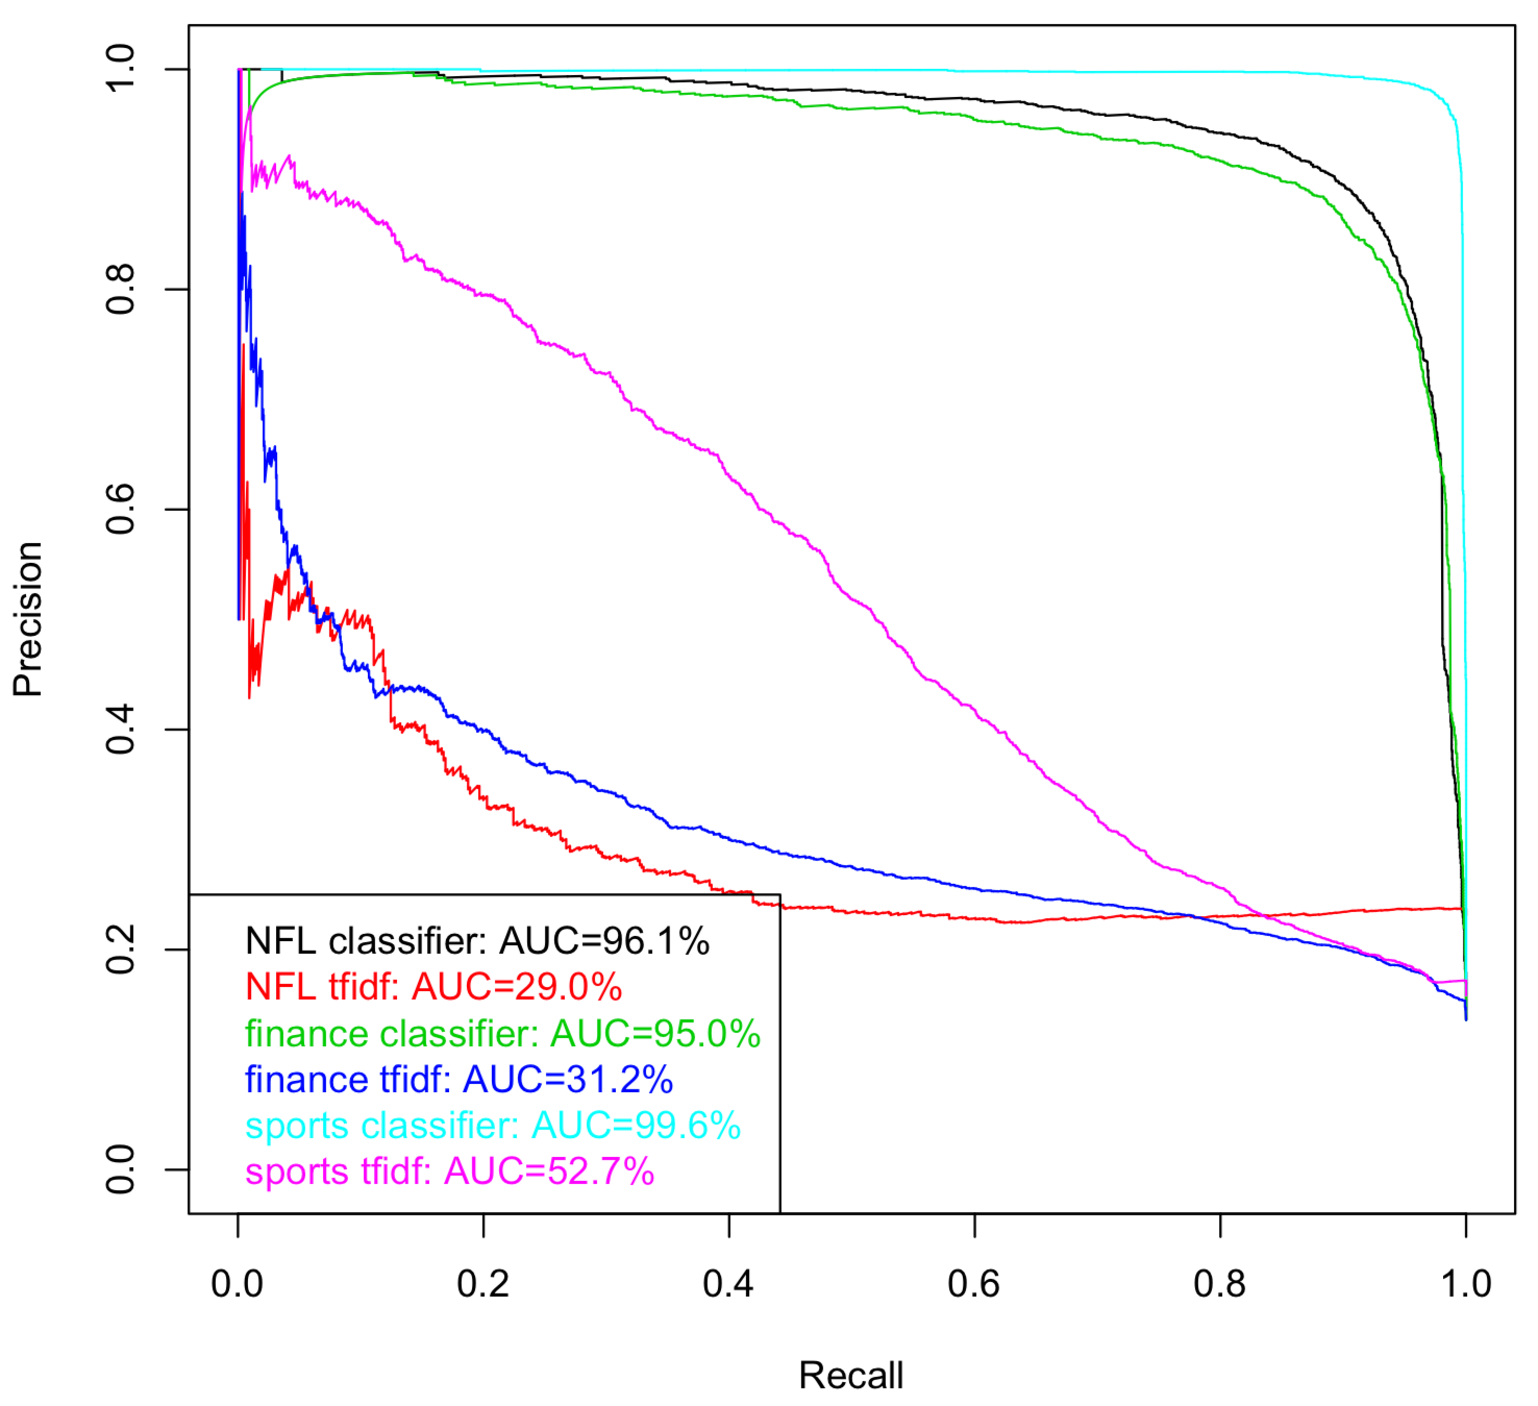
\includegraphics[scale=0.3]{precision-recall6.pdf}

\end{figure}


\subsubsection{Phase 1}

\begin{figure}[H]
\centering
\caption{Sports ROC} \label{Sports ROC}
\includegraphics[scale=0.3]{Sports-ROC.pdf}

\end{figure}
\begin{figure}[H]
\centering
\caption{Finance ROC} \label{Finance ROC}
\includegraphics[scale=0.3]{Finance-ROC.pdf}

\end{figure}
\label{tag:phase1exp}

\begin{table}
\caption{Phase 1 multiple models}
\begin{tabular}{|l|l|l|}
\hline
Method & Sports AUC & Finance AUC\\ \hline
gmp only & 0.58 & 0.62 \\ \hline
flat + gmp & 0.61 & 0.61 \\ \hline
SRQ + gmp & 0.62 & 0.63 \\ \hline
SRQ prune + gmp & 0.64 & 0.65 \\ \hline
\end{tabular}
\label{phase1exp2}
\end{table}


Here we present the ROC AUC for Sports and Finance under four sets of training methodologies (Table~\ref{tag:phase1exp}).  The ROC curves for the two streams are displayed in Figure~\ref{Sports ROC} and Figure~\ref{Finance ROC}. The weights for the consolidated components (gmp, $\langle \bfu, \bfq \rangle$, etc) are optimized a second time with respect to the training set. It is interesting to observe that the SRQ with negative regressor pruning results in an ROC curve that dominates all other models in both cases. We modified the exponential recency in the original dot product model in favor of a completely linear one, to achieve optimal ranking performance.


\begin{enumerate}
\item gmp only: $\rm{score} = \alpha \rm{gmp} + \beta \Delta T$;
\item flat dot-product (no SRQ) + gmp (baseline): $\rm{score} = \alpha_0 \rm{gmp} + \alpha_1 \langle \bfu,\bfd\rangle + \beta \Delta T$;
\item SRQ + gmp: $\rm{score} = \alpha_0 \rm{gmp} + \alpha_1 \langle \bfq \circ \bfu, \bfd \rangle + \beta \Delta T$;
\item SRQ with negative pruning + gmp: $\rm{score} = \alpha_0 \rm{gmp} + \alpha_1 \langle \widetilde{\bfq} \circ \bfu, \bfd \rangle + \beta \Delta T$, where $\widetilde{\bfq}_i = 0$ if $\bfq_i \le 0$.
\end{enumerate}








\subsubsection{phase 2}
\input phase2exp

%\subsubsection{Phase 3}
%
%
%
%We illustrate the results in Figure~\ref{DD curve} with a single user session. 
%\begin{figure}[H]
%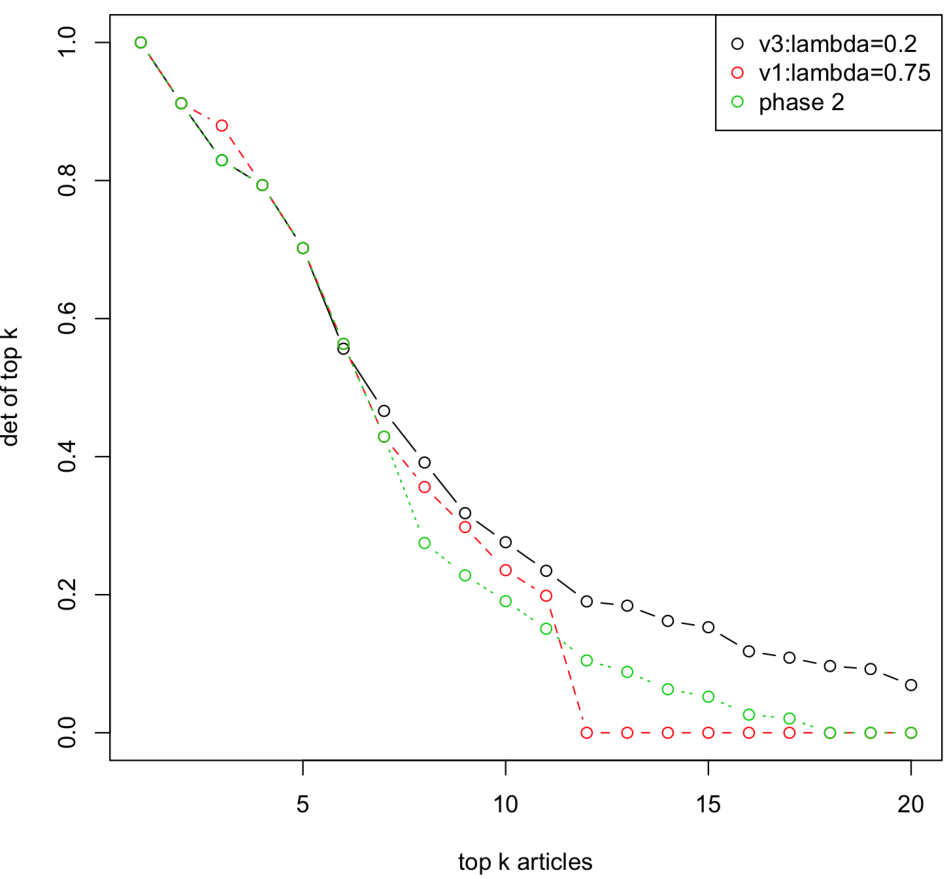
\includegraphics[scale=0.4]{DDcurve.pdf}
%\caption{Determinantal Diversity Curve}\label{DD curve}
%\end{figure}
%
%\begin{figure}[H]
%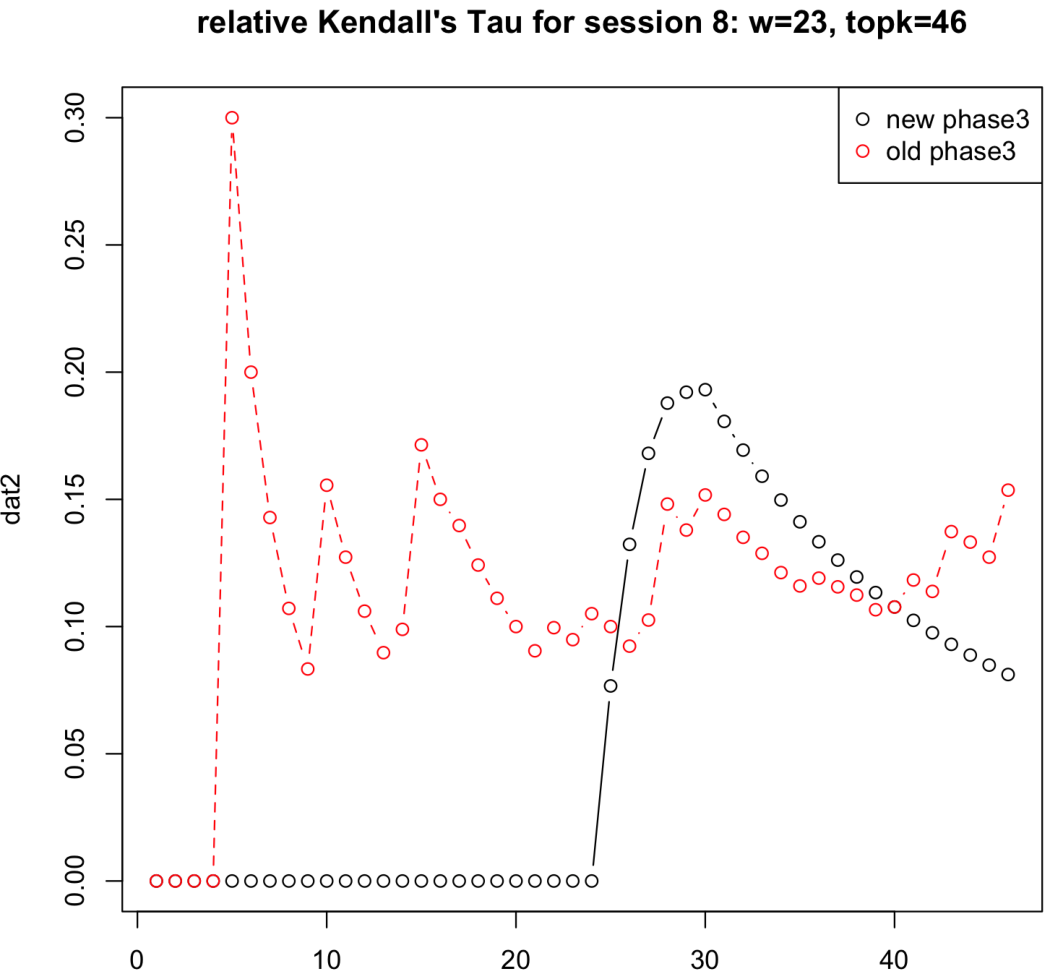
\includegraphics[scale=0.4]{KTcurve.pdf}
%\caption{Kendall's Tau Curve}
%\end{figure}
%
%In terms of determinantal diversity, algorithm v3 outperforms v1 (so-called MMR approach) or with no diversity at all, consistently across all top k positions, with only one exception at position 3. More importantly, by design v3 preserves the original order from phase 2 ranking up to the end of the first window limit, thus the Kendall's metric is flat at 0 for the duration of the first window. After the first window is exceeded, there is a momentary spike in top k Kendall tau metric, followed by rapid decrease to a level below that of v1. 
%
%\appendix
%\section{Diversity Ranking Results} \label{appendix diversity}
%Here we present the top 24 articles ranked by both algorithms v1 and v3 for a randomly chosen session on the Finance stream.
%
%Ranking of finance articles according to algorithm v1:
%\ssmall{
%\begin{verbatim}
%ph2    ph3    headline
%0       0       Carl Icahn says sellers 'completely misinterpreted' Apple's results"
%1       1       Bad Sign for Yahoo: Alibaba's Growth Slows"
%2       2       Steady Fed policy could steady markets"
%4       3       Indonesia Stocks Rise Most in 2 Weeks on Morgan Stanley Upgrade"
%3       4       Electronic Arts Sales Come Up Short in Console Transition"
%11      5       NYSE stocks posting largest volume increases"
%8       6       Ezcorp 1Q results top views, shares jump"
%7       7       VMware Falls 5%: Q1 Rev View In-Line, Year Rev View Beats"
%9       8       AT&T swings to 4th-quarter profit of $6.9 billion on higher revenue"
%14      9       AT&T reports profit on pension gain"
%13      10      Amgen earnings beat forecasts, but 2014 outlook leaves investors cold"
%16      11      AT&T revenue rises in fourth quarter"
%26      12      Check Point Advances to 12-Year High as Earnings Beat Estimates"
%23      13      Seagate Technology Earnings Miss In Difficult Market"
%15      14      Stocks End Higher; Data, Earnings in Focus"
%28      15      Why Swift Transportation (SWFT) Is Rising Today"
%38      16      Dow Today: E.I. Du Pont De Nemours & Company (DD) Lower"
%43      17      Remaking star fund managers to fit inside an ETF"
%29      18      Builders Rise On D.R. Horton Earnings, Home Prices"
%20      19      Stocks Higher In Afternoon; Polaris Trips Sell Rule"
%34      20      Rent-A-Center shares fall on disappointing 4Q"
%52      21      China Credit Repays Principal to Investors of Bailed-Out Trust"
%53      22      Sumitomo Mitsui Quarterly Profit Falls 9.3% on Bond-Trading Drop"
%37      23      Chipotle Earnings Seen Heating Up On Expansion Plans"
%\end{verbatim}}
%
%Ranking of the same 200 articles according to v3 (lambda = 0.10, w=24):
%\ssmall{
%\begin{verbatim}
%ph2    v3    headlines
%0       0       Carl Icahn says sellers 'completely misinterpreted' Apple's results
%1       1       Bad Sign for Yahoo: Alibaba's Growth Slows
%2       2       Steady Fed policy could steady markets
%3       3       Electronic Arts Sales Come Up Short in Console Transition
%4       4       Indonesia Stocks Rise Most in 2 Weeks on Morgan Stanley Upgrade
%7       5       VMware Falls 5%: Q1 Rev View In-Line, Year Rev View Beats
%8       6       Ezcorp 1Q results top views, shares jump
%9       7       AT&T swings to 4th-quarter profit of $6.9 billion on higher revenue
%10      8       NYSE stocks posting largest volume decreases
%13      9       Amgen earnings beat forecasts, but 2014 outlook leaves investors cold
%23      10      Seagate Technology Earnings Miss In Difficult Market
%26      11      Check Point Advances to 12-Year High as Earnings Beat Estimates
%28      12      Why Swift Transportation (SWFT) Is Rising Today
%29      13      Builders Rise On D.R. Horton Earnings, Home Prices
%34      14      Rent-A-Center shares fall on disappointing 4Q
%37      15      Chipotle Earnings Seen Heating Up On Expansion Plans
%38      16      Dow Today: E.I. Du Pont De Nemours & Company (DD) Lower
%41      17      American Airlines posts $2 billion loss on charges
%43      18      Remaking star fund managers to fit inside an ETF
%49      19      Maruti Net Income Misses Estimates After Discounts
%52      20      China Credit Repays Principal to Investors of Bailed-Out Trust
%53      21      Sumitomo Mitsui Quarterly Profit Falls 9.3% on Bond-Trading Drop
%54      22      What to expect from Obamacare bellwether Wellpoint
%61      23      [video] Why hedging will be key this year
%\end{verbatim}}
%
%Version 1 often does not properly eliminate articles with very similar content, judging from their headlines, as  the three almost back-to-back AT\&T articles demonstrate. Equally serious is the observation that many articles under v1 get reversed in their relative order for no apparently good reason. The minimally disruptive nature of v3 makes it an at least locally optimal meta-algorithm on top of phase 2 gbdt ranking.
%
% The following two commands are all you need in the
% initial runs of your .tex file to
% produce the bibliography for the citations in your paper.

\section{Conclusions}
\label{sec:conclusions}
This paper describes a system to recommend contents for multiple semantic 
streams.
%Web portal provides contents for users to browse. 
 We present a semantic stream hierarchy to guide internet users to  browse 
 contents and help them find personally interesting articles more easily and 
 quickly. To solve the content recommendation problem for multiple semantic 
 streams at various depths, we face unique challenges such as scalable 
 multi-layer stream classification and stream ranking. 

% We all know content recommendation is very different from Web search engine.  Search engine provides search results for an issued query, but web portal recommends %content without query. Instead,  users browse the contents. To serve user browse,  In order to solve content recommendation for multiple semantic streams,   not only do we %experience the same challenges as existing work such as recency, and personalization, but we are facing new challenges that 

Several new methods are proposed such as click-based stream classifier and 
using stream-id to improve multiple stream ranking.  All these methods are 
found effective and improved upon baseline model significantly.  

%Our work also presented new results regarding recency handling. Experiments suggest that both relevance and recency were improved, which is a significant progress over the %results of existing work ~\cite{Liu:2010:PNR:1719970.1719976}.  

The whole system is decomposed into three phases: phase 0 as a multi-stream 
classifier and phase 1 and phase 2 as ranking models. Phase 0 can arguably be 
combined with phase 1, since both have linear forms. This is the spirit of 
model Eq.~\eqref{original SRQ}. In practice, however, we find the latency
unacceptable when applying the combined algorithm at serving time, since 
document profiles can have significantly more features than users. Instead, 
phase 0 
takes away some of the burden in Eq.~\eqref{original SRQ} by computing the 
document-only component scores during content ingestion time, and a simplified 
phase 1 model Eq.~\eqref{practical SRQ} is adopted for fast document retrieval.

We demonstrate order of magnitude improvement in precision-recall of the 
linear classifier over tfidf approach. Compared with hand-crafted rule-based 
approach, the classifier significantly increases recall while maintaining the 
same or better precision. For phase 1 personalized stream-specific linear 
ranking, we measure the performance in terms of click/skip ROC curves and show 
an increase in Area Under the Curve (AUC) of 3-4\% under model 
Eq.~\eqref{practical SRQ}  over the stream-independent model. Finally phase 2 
refines the ranking results from phase 1 by taking into account a select set 
of 14 features related to user, document, and their interactions. We observe 
huge CTR and dwell-time gains over the baseline from online user experience 
test.




%Our approaches to solve semantic stream recommendation are effective.  There are some popular approaches such as explore/exploit for news recommendation. These %methods are useful for a single stream, but not scalable for multiple streams like ours.  To design a recommendation system we must consider system latency. Explore/exploit %strategy is not suitable for this task. But we exploited the idea of exploration bucket to collect unbiased training data. Our 3-phase structure recommendation is available to %recommend articles from thousands of articles in mil-second scale.







%The exact metric definitions are reviewed in Section~\ref{evaluation metrics}.

To summarize, we design a highly efficient, scalable stream content recommendation system that optimizes user experience measured in terms of CTR, by seeking a balance among the following four desirable attributes: relevance (to the individual stream), popularity, freshness, and personalization.


 In practice, not all 3 phases are applied to all streams uniformly. Some 
 small streams have few articles, or may not need 
 personalization from Phase 1 or Phase 2.  It is flexible to 
 adjust the 3 phases for different steams. This will be examined in an 
 upcoming work.





\bibliographystyle{abbrv}
\bibliography{gs-ranking,ref1,ref3}  % sigproc.bib is the name of the Bibliography in this case






% comments for how to generate the plots in R
\/*
~/Documents/latex/grandslam/plots/

plot(c(0,1),c(0,1),type="n", xlab='Recall', ylab='Precision');

g=file('fin.c=10.predlab');
f=read.table(g);
names(f) = c('pred','label');
library('ROCR');
pred <- prediction(f$pred,f$label);
perf <- performance(pred,'prec','rec');
plot(perf,add=T,col=1);

g=file('fin.tfidf.predlab');
f=read.table(g);
names(f) = c('pred','label');
library('ROCR');
pred <- prediction(f$pred,f$label);
perf <- performance(pred,'prec','rec');
plot(perf,add=T,col=2);

g=file('spt.c=10.predlab');
f=read.table(g);
names(f) = c('pred','label');
library('ROCR');
pred <- prediction(f$pred,f$label);
perf <- performance(pred,'prec','rec');
plot(perf,add=T,col=3);

g=file('spt.tfidf.predlab');
f=read.table(g);
names(f) = c('pred','label');
library('ROCR');
pred <- prediction(f$pred,f$label);
perf <- performance(pred,'prec','rec');
plot(perf,add=T,col=4);

g=file('nflspt.c=10.predlab');
f=read.table(g);
names(f) = c('pred','label');
library('ROCR');
pred <- prediction(f$pred,f$label);
perf <- performance(pred,'prec','rec');
plot(perf,add=T,col=5);

g=file('nflspt.tfidf.predlab');
f=read.table(g);
names(f) = c('pred','label');
library('ROCR');
pred <- prediction(f$pred,f$label);
perf <- performance(pred,'prec','rec');
plot(perf,add=T,col=6);


legend(0,0.25,c('finance classifier: AUC=99.8%','finance tfidf: AUC=31.2%','sports classifier: AUC=99.9%','sports tfidf: AUC=52.7%', 'nfl classifier: AUC=96.3%','nfl tfidf: AUC=29.0%'),text.col=c(1,2,3,4,5,6));

*/

% compute precision recall from a prediction-label space separated file
\/*
#!/bin/bash
# computes pointwise precision recall at 0 threshold
file=$1
pos=`cat $file | awk '{if ($1 > 0) print $0}' | wc -l`
neg=`cat $file | awk '{if ($1 < 0) print $0}' | wc -l`
truepos=`cat $file | awk '{if ($1 > 0 && $2 == 1) print $0}' | wc -l`
trueneg=`cat $file | awk '{if ($1 < 0 && $2 == -1) print $0}' | wc -l`
falsepos=$(( pos - truepos ))
falseneg=$(( neg - trueneg ))
precision=`echo "$truepos / $pos" | bc -l`
recall=`echo "$truepos / ( $truepos + $falseneg )" | bc -l`
echo "precision = " $precision
echo "recall = " $recall
*/



\end{document}
